\section{Electron Matter Interactions}
To understand the interactions between electrons and matter, it is 
necessary to introduce some terminology.
\textit{Primary electrons} are electrons which are emitted directly from
the cathode and head to the sample.
After arriving at the surface, the electrons undergo elastic and inelastic scattering.
Due to complex interactions between the primary electrons and the atoms 
inside the sample, multiple interaction products are generated, which can
be classified into different catagories. 
The catagories, that are relevant for conducing the experiment are the 
following:
\begin{itemize}
	\item Secondary electrons
	\item Backscattered electrons
	\item X-Ray emission
	\item Cathodoluminescence
\end{itemize}
After arriving at the surface, the electrons spread due to 
small-angle scattering in a pear shaped area around the collision point. 
This is visualizied in \cref{fig:birne}.
\begin{figure}[H] 
	\centering
	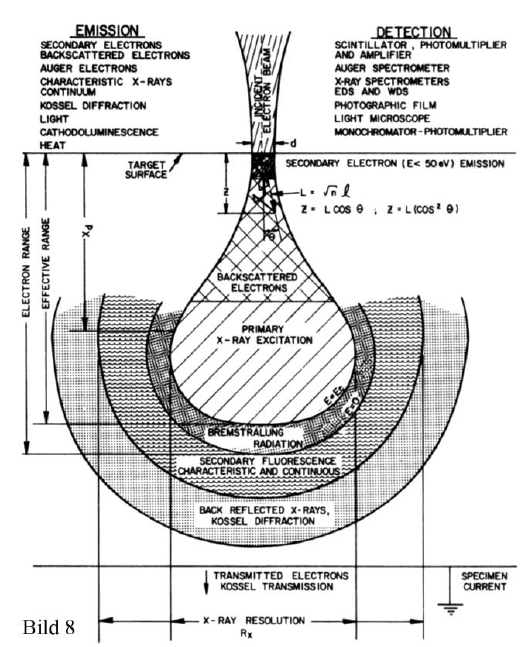
\includegraphics[width=0.95\linewidth]{../assets/birne.png}
	\caption{interaction area of electrons}
	\label{fig:birne}
\end{figure}


